\documentclass[a4paper]{report} % set paper size

\usepackage[utf8]{inputenc}
\usepackage {url}
\usepackage[top=2.0cm, bottom=2.0cm, left=2.54cm, right=2.54cm]{geometry} % set margin
\usepackage{amsfonts} % for set names
\usepackage{amsmath} % for equation system
\usepackage{amsthm} % for theorem block
\usepackage{fixltx2e} % for subscript
\usepackage{fancyhdr} % for footer/headline modification
\usepackage{xcolor}
\usepackage{graphicx} % for image insertion
\usepackage[ruled,vlined]{algorithm2e} % for algorithm integration

\pagestyle{fancyplain} % for footing modification on all pages
\fancyhf{}
%\renewcommand{\headrulewidth}{0pt} % remove decorative lign
\fancyhead[L]{Alexandre Devienne}
\fancyhead[R]{EL-BA1 EPFL 2014}
\fancyhead[C]{\textbf{Autumn programming project : Recolor}}

\fancyfoot[R]{\thepage\ of \pageref{lastpage}}

\begin{document}

\section{Program's architecture}
\begin{figure}
\begin{center}
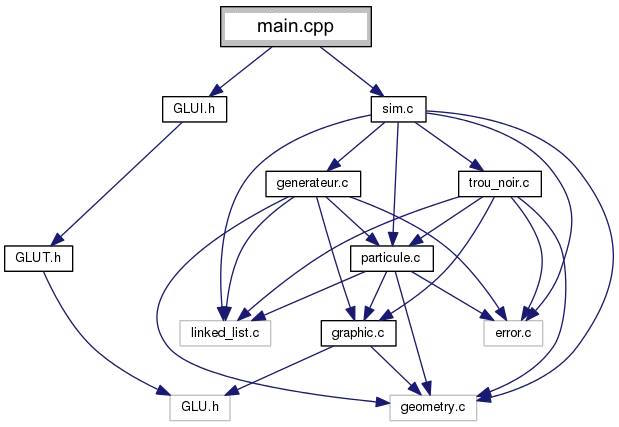
\includegraphics[scale=0.6]{architecture.jpg}
\end{center}
\caption{Final arhcitecture}
\end{figure}


\section{Data structures}

\section{Function called by \text{main.cpp} from \text{sim.c}

\label{lastpage}
\end{document}
